%% LyX 2.1.4 created this file.  For more info, see http://www.lyx.org/.
%% Do not edit unless you really know what you are doing.
\documentclass[english]{article}
\usepackage[T1]{fontenc}
\usepackage[latin9]{inputenc}
\usepackage{textcomp}
\usepackage{graphicx}

\makeatletter

%%%%%%%%%%%%%%%%%%%%%%%%%%%%%% LyX specific LaTeX commands.
%% Because html converters don't know tabularnewline
\providecommand{\tabularnewline}{\\}

\makeatother

\usepackage{babel}
\begin{document}

\part*{Gentrification index measure}

There is no general accepted definition of ``gentrification''. The
term was coined by British sociologist Ruth Glass in 1964. She was
describing the displacement of lower-class worker residents in urban
neighborhoods by middle-class people in Islington, London\cite{gentrification_def}.
This vague and abstract definition makes it even harder to measure
the extent of gentrification of a whole city quantitatively.

The idea behind getting a number for the ``amount'' of gentrification
happening in a city is to merely focus on the change of the household
income with respect to time. All other census data, which claim to
measure gentrification, can be viewed as its effects according to
\cite{gentr_causes}. Hence, we decided to divide a city into districts
by virtue of the town subdivision (???), and compared the median household
income per month (MHI) of each district from data 10 years apart.
To assure that the increase is free from inflation and other economic
growth factors we calculate the increase of MHI in each district $x_{i}=x(i=District)$
relative to the increase of the mean MHI of the whole city $\tilde{x}$.
More precisely, 
\begin{equation}
x_{i}=\frac{\mathrm{MHI}(i,2016)-\mathrm{MHI}(i,2007)}{\mathrm{MHI}(i,2016)},\quad\tilde{x}=\frac{\widehat{\mathrm{MHI}}(2016)-\widehat{\mathrm{MHI}}(2007)}{\widehat{\mathrm{MHI}}(2016)},\label{eq:mhi}
\end{equation}
where $\ \widehat{}\ $ denotes the average of MHI in a particular
year over all districts $i$. Then we use $\tilde{x}$ as a reference
for the increase $x_{i}$. Tab.$\,$\ref{tab:Median-household-income}
shows this ``relative'' increase of the MHI, $r_{i}=\left(x_{i}-\tilde{x}\right)/\tilde{x}$,
in case of Berlin. Furthermore, we are also interested in the change
of the number of household $H_{i}=\mathrm{N}(i,2016)/\mathrm{N}(i,2007)$
in a certain district. This also influences gentrification. If, for
instance, rental fees increase but the number of household decrease
in a certain area, then we can assume that several cheaper households
were displaced by a few expensive ones. 

\begin{table}[h]
\begin{centering}
\begin{tabular}{|c|c|c|c|c|c|c|}
\hline 
District & $\frac{\mathrm{N}(i,2007)}{1000}$ & $\frac{\mathrm{N}(i,2016)}{1000}$ & $H_{i}$ & $\mathrm{MHI}(i,2007)$ & $\mathrm{MHI}(i,2016)$ & $r_{i}$ \tabularnewline
\hline 
\hline 
1 & $161.4$ & $152.0$ & $0.94$ & 1825 & 2325 & $-0.03$\tabularnewline
\hline 
2 & $119.3$ & $124.4$ & $1.04$ & 1550 & 1775 & $-0.43$\tabularnewline
\hline 
3 & $199.7$ & $182.5$ & $0.91$ & 1575 & 2125 & $+0.16$\tabularnewline
\hline 
4 & $125.9$ & $133.0$ & $1.06$ & 1675 & 2025 & $-0.22$\tabularnewline
\hline 
5 & $187.8$ & $212.3$ & $1.13$ & 1425 & 1825 & $-0.01$\tabularnewline
\hline 
6 & $189.4$ & $183.5$ & $0.97$ & 1575 & 1975 & $-0.09$\tabularnewline
\hline 
7 & $173.5$ & $164.7$ & $0.95$ & 1175 & 1800 & $+0.56$\tabularnewline
\hline 
8 & $218.8$ & $214.9$ & $0.98$ & 1525 & 2150 & $+0.31$\tabularnewline
\hline 
9 & $166.4$ & $169.8$ & $1.02$ & 1350 & 1700 & $-0.07$\tabularnewline
\hline 
10 & $141.9$ & $159.5$ & $1.12$ & 1450 & 1825 & $-0.08$\tabularnewline
\hline 
11 & $127.9$ & $132.8$ & $1.04$ & 1525 & 1950 & $-0.07$\tabularnewline
\hline 
12 & $128.9$ & $134.6$ & $1.04$ & 1625 & 2050 & $-0.07$\tabularnewline
\hline 
\end{tabular}
\par\end{centering}

\caption{Median household income per month in EUR in Berlin (city divided into
districts according to Fig.$\,$\ref{fig:Map-of-Berlin's}) in years
2007 \& 2016.\label{tab:Median-household-income}}
\end{table}


The next step is to define a measure for the distance of a district
with respect to each other. A generic solution is to use the underling
structure of an city, the districts itself as distance units. Therefore,
we introduce the number of minimal district-border-crossings, which
are necessary to get from district $i$ to district $j$, as our distant
measure. For example, the distance, denoted as $\left\langle \cdot,\cdot\right\rangle $,
of district 1 to district 8 in Fig.$\,$\ref{fig:Map-of-Berlin's}
is equal to 3, i.e. $\left\langle 1,8\right\rangle =3$. Hence, differences
in the values $r_{i}$ of district further apart contribute less to
the gentrification index $g_{i}$ of an particular district $i$.

To compute the distances of the districts from a map in this measure,
we applied ... ??? (a technique from graph theory / machine learning)
...

\begin{figure}
\centering{}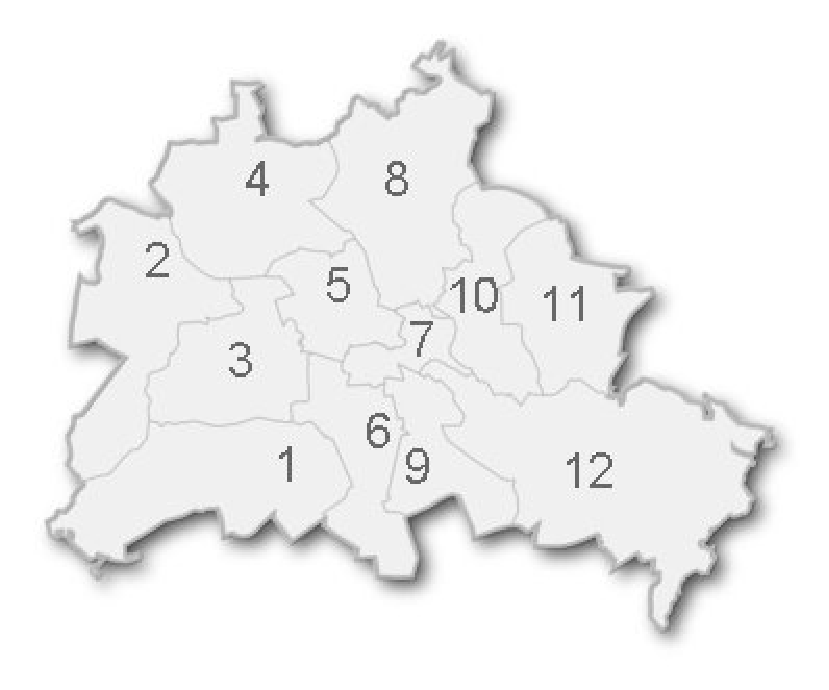
\includegraphics[scale=0.6]{stadtplan-berlin}\caption{Map of Berlin's districts with random numbering. Image: � Increa\label{fig:Map-of-Berlin's}}
\end{figure}


The final step consists of putting the quantities $\left\langle \cdot,\cdot\right\rangle $
and $r_{i}$ together in a way which results in a meaningful measure
of gentrification. We propose that the following formula is a comprehensive
quantity to measure the gentrification of a city, 
\begin{equation}
G=\sum_{i=1}^{N}\frac{G_{i}}{H_{i}},\quad G_{i}=\sum_{j=1,\,j\neq i}^{N}\frac{\left|r_{i}-r_{j}\right|^{2}}{\left\langle i,j\right\rangle ^{2}}.\label{eq:gindex}
\end{equation}
We call $G$ and $G_{i}$ the gentrification index of a city and the
gentrification index of the city district $i$ respectively. Due to
the fact that gentrification is a rather subjective notion, and the
fact that in the perspective of citizens it manifests itself the most
when adjacent neighborhoods are compared, we take the square of our
distance measure $\left\langle \cdot,\cdot\right\rangle $. This has
the effect to soften the differences between two districts when they
are far apart. The meaning of the numerator in Eq.$\,$(\ref{eq:gindex})
is clear when we write out the squares, $\left(x_{i}^{2}-x_{j}^{2}\right)/\tilde{x}^{2}.$
The numerator is smaller, if the mean MHI of the city $\tilde{x}$
is high. Then, two district with a big difference in the MHI $x_{i}-x_{j}$
are going to make $G_{i}$ small, whereas on those where the difference
is small $\tilde{x}$ has no effect at all. With this feature we can
take into account the overall increase of the MHI in a city. The gentrification
index of an city with a low $\tilde{x}$ but a distinctive shift of
citizens of different working-classes shall be especially big, as
we can then assume that wealthier people haven't moved in from beyond
the city at an above average rate.

Although, the above argumentation is sensible, we can't be sure if
(\ref{eq:gindex}) is the best formula for the index. Thus, we also
present some alternatives to $G_{i}$, and compare these to Eq.$\,$(\ref{eq:gindex}).
Namely,
\begin{equation}
\begin{array}{cc}
G_{i}^{\prime}= & \sum_{j=1,\,j\neq i}^{N}\frac{\left|r_{i}-r_{j}\right|^{2}}{\left\langle i,j\right\rangle }\\
G_{i}^{\prime\prime}= & \sum_{j=1,\,j\neq i}^{N}\frac{\left|r_{i}-r_{j}\right|}{\left\langle i,j\right\rangle ^{2}}\\
G_{i}^{\prime\prime\prime}= & \sum_{j=1,\,j\neq i}^{N}\frac{\left|r_{i}-r_{j}\right|}{\left\langle i,j\right\rangle }
\end{array}.\label{eq:gindex_alt}
\end{equation}
Tab.$\,$\ref{tab:Correlation} shows the correlation between the
gentrification indexes in each district and the quantities $r_{i},H_{i}$
for the various types of $G_{i}$, and the gentrification index $G$
as well. Based on this result we propose the formula in Eq.$\,$(\ref{eq:gindex})
as our best measure for the gentrification of a city.

\begin{table}[h]
\begin{centering}
\begin{tabular}{|c|c|c|c|c|}
\hline 
$G$ & $8.85$ & $11.20$ & $18.52$ & $23.54$\tabularnewline
\hline 
\hline 
$\mathrm{corr}\left(\cdot,\cdot\right)$ & $G_{i}$ & $G_{i}^{\prime}$ & $G_{i}^{\prime\prime}$ & $G_{i}^{\prime\prime\prime}$\tabularnewline
\hline 
$r_{i}$ & $0.39$ & $0.35$ & $0.33$ & $0.28$\tabularnewline
\hline 
$H_{i}$ & $0.77$ & $0.78$ & $0.85$ & $0.86$\tabularnewline
\hline 
\end{tabular}
\par\end{centering}



\caption{Correlation\label{tab:Correlation}}


\end{table}


\begin{thebibliography}{99}
\bibitem{gentrification_def} Ruth Glass (1964). London: aspects of change. London: MacGibbon \& Kee.
\bibitem{gentr_causes} Steve Holland, Gentrification: Causes and Consequences, Journal of Lutheran Ethics, Vol. 16, Issue 1, Jan 2016
\end{thebibliography}
\end{document}
